\section{Feature Extraction for Coq terms}\label{sec:lemmaclustering}

ML4PG uses (unsupervised) \emph{clustering algorithms}~\cite{Bishop} to find patterns in Coq syntax and proofs.
Clustering algorithms
divide data into $n$ groups of similar objects (called \emph{clusters}), where the value of $n$
is a parameter provided by the user. In ML4PG, the value of $n$ is automatically computed depending on the number
of objects to cluster, and using the formula provided in~\cite{KHG13,lpar13}.
A detailed exposition of machine-learning algorithms involved in ML4PG can be found in \cite{KHG13}. In this paper, our first goal consists in improving ML4PG's feature extraction algorithm.


\emph{Feature extraction}~\cite{Bishop} is a research area developing methods for
discovery of statistically significant features in data.
We adopt the following standard terminology.
We assume there is a training data set, containing some samples (or objects).
\emph{Features} are given by a set of statistical parameters chosen to represent all objects in the given data set.
If $n$ features are chosen, one says that object classification is
conducted in an $n$-dimensional space.
For this reason, most pattern-recognition tools will require that
the number of selected features is limited and fixed (sparse methods, like the ones applied in
e.g.~\cite{lpar-urban,K13,UrbanSPV08} are the exception to this rule).
\emph{Feature values} are rational numbers used to instantiate the features for every given object.
If an object is characterised by $n$ feature values, these $n$ values together form a \emph{feature vector} for this object.
A function that assigns, to every object of the data set, a feature vector is called a \emph{feature extraction function}.
Normally, feature extraction is a data pre-processing stage, and it is separated from the actual pattern-recognition process.


Feature extraction from terms or \emph{term trees} is common to most feature extraction algorithms implemented
in theorem provers~\cite{lpar13,lpar-urban,K13,UrbanSPV08}. In~\cite{lpar13}, we introduced a feature extraction mechanism
for ACL2 first-order terms. Here, that ACL2 method is substantially re-defined to capture the higher-order dependently-typed language of Coq.


The underlying formal language of Coq is known as the \emph{Predicative Calculus of (Co)Inductive Constructions} (pCIC)~\cite{Coq,CoquandH88,CoPa89}.
The terms of pCIC are built from
the following rules:


\begin{definition}[pCIC term]\label{def:coqterms}

$-$ The sorts \lstinline?Set?, \lstinline?Prop?, \lstinline?Type(i)? (\lstinline?i?$\in \mathbb{N}$) are terms.

$-$ The global names of the environment are terms.

$-$ Variables are terms.

$-$ If \lstinline?x? is a variable and \lstinline?T, U? are terms, then \lstinline?forall x:T,U?
 is a term. If \lstinline?x? does not occur in \lstinline?U?, then \lstinline?forall x:T,U? will be written as \lstinline?T -> U?. A term of the
 form \lstinline?forall x1:T1, forall x2:T2, ..., forall xn:Tn, U? will be written as \lstinline?forall (x1:T1) (x2:T2) ...(xn:Tn), U?.

$-$ If \lstinline?x? is a variable and \lstinline?T, U? are terms, then \lstinline?fun x:T => U?
 is a term. A term of the form \lstinline?fun x1:T1 => fun x2:T2 => ... => fun xn:Tn => U? will be written as \lstinline?fun (x1:T1) (x2:T2) ...(xn:Tn) => U?.

 $-$ If \lstinline?T? and \lstinline?U? are terms, then \lstinline?(T U)? is a term -- we use an uncurried notation (\lstinline?(T U1 U2 ... Un)?)
 for nested applications (\lstinline?(((T U1) U2) ... Un)?).

 $-$ If \lstinline?x? is a variable, and \lstinline?T, U? are terms, then (\lstinline?let x:=T in U?) is a term.

\end{definition}

The syntax of Coq terms~\cite{Coq} includes some terms that do not appear in Definition~\ref{def:coqterms}; e.g. given
 a variable \lstinline?x?, and  terms \lstinline?T? and \lstinline?U?, \lstinline?fix name (x:T) := U? is a Coq term used to declare a recursive definition.
The notion of a term in Coq covers a very general syntactic
category in the Gallina specification language~\cite{Coq} and corresponds to the intuitive notion of well-formed expression.
However, for the purpose of concise exposition,
we will restrict our notion of a term to Definition~\ref{def:coqterms},
giving the full treatment of the whole Coq syntax in the actual ML4PG implementation.


\begin{definition}[ML4PG term tree]\label{def:ml4pgtermtree}
Given a Coq term \lstinline?C?, we define its associated term tree as follows:

$-$ If \lstinline?C? is one of the sorts \lstinline?Set?, \lstinline?Prop? or \lstinline?Type(i)?, then the term tree of
 \lstinline?C? consists of one single node, labelled respectively by \lstinline?Set:Type(0)?, \lstinline?Prop:Type(0)? or \lstinline?Type(i):Type(i+1)?.

$-$ If \lstinline?C? is a name or a variable, then
 the term tree of \lstinline?C? consists of one single node, labelled by the name or the variable itself together with its type.

$-$ If \lstinline?C? is a term of the form \lstinline?forall (x1:T1) (x2:T2) ...(xn:Tn), U? (analogously for \lstinline?fun (x1:T1) (x2:T2) ...(xn:Tn) => U?);
then, the term tree of \lstinline?C? is the tree with the root node labelled by \lstinline?forall? (respectively \lstinline?fun?)
and its immediate subtrees given by the trees representing \lstinline?x1:T1?, \lstinline?x2:T2?, \lstinline?xn:Tn? and \lstinline?U?.

$-$ If \lstinline?C? is a term of the form \lstinline?let x:=T in U?, then the term tree of \lstinline?C?
 is the tree with the root node labelled by \lstinline?let?, having three subtrees given by the trees corresponding to \lstinline?x?, \lstinline?T? and \lstinline?U?.


$-$ If \lstinline?C? is a term of the form  \lstinline?T -> U?, then  the term tree of \lstinline?C?  is represented by the tree with the root node labelled by
\lstinline?->?, and its immediate subtrees given by the trees representing  \lstinline?T? and \lstinline?U?.

$-$ If \lstinline?C? is a term of the form  \lstinline?(T U1 ... Un)?, then we have two cases.
If \lstinline?T? is a name, the term tree of \lstinline?C?  is represented by
the tree with the root node labelled by \lstinline?T? together with its type, and its immediate subtrees given by the trees
representing \lstinline?U1?,\ldots, \lstinline?Un?. If \lstinline?T? is not a  name, the term tree of \lstinline?C?
is the tree with the root node labelled by \lstinline?@?, and its immediate subtrees given by the trees
representing \lstinline?T?, \lstinline?U1,...,Un?.


\end{definition}


Note that ML4PG term trees consist of two kinds of nodes: \emph{Gallina} and \emph{term-type} nodes. The Gallina nodes are
labelled by Gallina-keywords and special tokens such as \lstinline?forall?, \lstinline?fun?, \lstinline?let? or \lstinline?->? (from now on, we will call them Gallina tokens);
and the term-type nodes are labelled by expressions of the form \lstinline?t1:t2? where \lstinline?t1? is a sort, a variable or
a name, and  \lstinline?t2? is the type of \lstinline?t1?.


\begin{figure}[t]
\centering
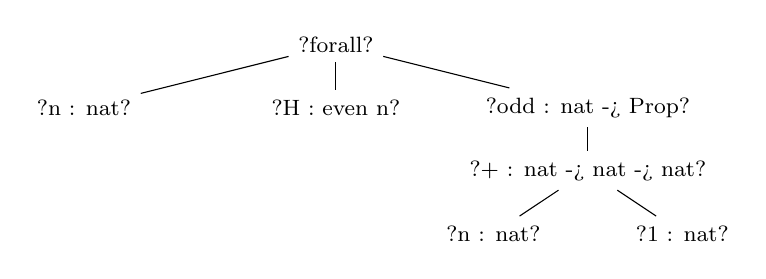
\begin{tikzpicture}[level 1/.style={sibling distance=40mm},
 level 2/.style={sibling distance=70mm},
 level 3/.style={sibling distance=30mm},
 level 4/.style={sibling distance=30mm},scale=.8,font=\footnotesize]

   \node (root) {\lstinline?forall?} [level distance=10mm]
             child { node {\lstinline?n : nat?}}
             child { node {\lstinline?H : even n?}}
             child { node {\lstinline?odd : nat -> Prop?}
                      child { node {\lstinline?+ : nat -> nat -> nat?}
                           child { node {\lstinline?n : nat?}}
                           child { node {\lstinline?1 : nat?}}
                           }
                   }

    ;
 \end{tikzpicture}
\caption{\scriptsize{\emph{ML4PG term tree for the term \texttt{forall (n : nat) (H : even n), odd (n + 1).}}}}\label{fig:termtree}
\end{figure}

\begin{example}\label{ex1}
 Given the term \lstinline?forall (n : nat) (H : even n), odd (n + 1)?, its ML4PG term tree is depicted in Figure~\ref{fig:termtree}.
 \end{example}

We represent ML4PG term trees as feature matrices, further to be flattened into feature vectors for clustering.
A variety of methods exists to represent trees as matrices, for instance using
adjacency or incidence matrices. The adjacency matrix and the various previous methods of  feature
extraction (e.g.~\cite{lpar-urban,K13,UrbanSPV08}) share the following common properties: different
library symbols are represented by distinct features, and the
feature values are binary.
For
big libraries and growing syntax, feature vectors grow very large (up to $10^6$ in some experiments)
and at the same time very sparse, which implies the use of sparse machine-learning methods.

We develop a new compact method that tracks a large (potentially unlimited) number of Coq terms by a finite number of features and an unlimited number of feature-values.
In our method, the features are given by two properties common to all possible term trees: the term tree depth and the level index of nodes.
The most important information about the term is then encoded by improving precision of feature values
using rational-valued feature-extraction functions. Taking just $300$ features, the new feature-extraction method recursively adjusts the feature values,
adapting to the growing language syntax.
The resulting feature vectors have an average density ratio of 60\%.

Given a Coq expression, we can differentiate its term and type components; the feature values capture information from
these components and also the structure of the tree. In particular, each tree node is encoded by distinct feature values
given by a triple of rational numbers to represent the term component, the type component, and the level index of the parent node in the term tree,
cf. Table~\ref{ml4pgtermtable}. Our feature extraction method is formalised in the following definitions.

\begin{table}[t]
\tbl{\scriptsize{\emph{ML4PG term tree matrix for \texttt{forall (n : nat) (H : even n), odd (n+1)}.}}\label{ml4pgtermtable}}{
\centering
{\scriptsize
\begin{tabular}{|c||c|c|c|}
\hline
 &  level index 0 & level index 1 & level index 2 \\
 \hline
td0 & ($[\texttt{forall}]_{Gallina}$,-1,-1) & (0,0,0) & (0,0,0)\\
\hline
td1 & ($[\texttt{n}]_{term}$,$[\texttt{nat}]_{type}$,0) & ($[\texttt{H}]_{term}$,$[\texttt{even n}]_{type}$,0)& ($[\texttt{odd}]_{term}$,$[\texttt{nat-> Prop}]_{type}$,0) \\
\hline
td2 & ($[\texttt{+}]_{term}$,$[\texttt{nat -> nat -> nat}]_{type}$,2) & (0,0,0)& (0,0,0)\\
\hline
td3 & ($[\texttt{n}]_{term}$,$[\texttt{nat}]_{type}$,0) & ($[\texttt{1}]_{term}$,$[\texttt{nat}]_{type}$,0)  & (0,0,0)\\
\hline
\end{tabular}}}
\end{table}


\begin{definition}[Term tree depth level and level index]\label{def:termtreelevel}
Given  a term tree $T$, the \emph{depth} of the node $t$ in $T$, denoted by \emph{depth(t)}, is defined as follows:

$-$ $depth(t) = 0$, if $t$ is a root node;

$-$ $depth(t) = n+1$, where $n$ is the depth of the parent node of $t$.

The \emph{$n$th level} of $T$ is the ordered sequence of nodes of depth $n$ --- using the classical representation for trees, the order of the sequence is
given by visiting the nodes of depth $n$ from left to right. The \emph{level index} of a node with depth $n$ is the position of the node in the $n$th level of $T$.
We denote by $T(i,j)$ the node of $T$ with depth $i$ and index level $j$.
\end{definition}

We use the notation $M[\mathbb{Q}]_{n\times m}$ to denote the set of matrices of size  $n\times m$ with rational coefficients.


\begin{definition}[ML4PG term tree feature extraction]\label{df:matrix}
Given a term \lstinline?t?, its corresponding term tree $T_{\texttt{t}}$, and three injective functions
$[.]_{term}: Coq~terms \rightarrow \mathbb{Q}^+$, $[.]_{type}: Coq~terms \rightarrow \mathbb{Q}^+$
and $[.]_{Gallina}: Gallina~tokens \rightarrow \mathbb{Q}^-$, then the feature extraction function
$[.]_M=\langle[.]_{term}, [.]_{type},[.]_{Gallina}\rangle : Coq~terms \rightarrow M[\mathbb{Q}]_{10\times 10}$
builds the  \emph{term tree matrix of \texttt{t}}, $[\texttt{t}]_M$,
where the $(i,j)$-th entry of $[\texttt{t}]_M$ captures information from the node $T_{\texttt{t}}(i,j)$ as follows:

$-$ if $T_{\texttt{t}}(i,j)$ is a Gallina node $g$, then the $(i,j)$th entry of $[\texttt{t}]_M$ is a triple $([g]_{Gallina},-1,p)$
where $p$ is the level index of the parent of $g$.

$-$ if $T_{\texttt{t}}(i,j)$ is a term-type node \lstinline?t1:t2?, then the $(i,j)$th entry of $[\texttt{t}]_M$ is a triple $([t1]_{term},[t2]_{type},p)$
where $p$ is the level index of the parent of the node.




\end{definition}




In the above definition, we fix  the maximum depth and  maximum level index of a node to $10$; this makes the feature extraction mechanism uniform
across all Coq terms appearing in the libraries. We may lose some information if  pruning is needed, but the chosen size works well for most terms appearing in Coq libraries.
If a term tree does not fit into $10 \times 10$ term tree dimensions, its $10 \times 10$
subtree is still considered by ML4PG.
The term tree matrix is flattened into a feature vector, and each triple will be split
into three components of the vector, giving a feature vector size of $300$,
still smaller than in sparse approaches~\cite{lpar-urban,K13,UrbanSPV08}.


In Definition~\ref{df:matrix}, we deliberately specify the functions $[.]_{Gallina}, [.]_{term}$ and $[.]_{type}$ just by their signature.
The function $[.]_{Gallina}$ is a predefined function.
The number of Gallina tokens (\lstinline?forall?, \lstinline?fun?, \lstinline?->? and so on) is fixed and cannot be
expanded by the Coq user. Therefore, we know in advance all the Gallina tokens that can appear in a development, and we can
assign a concrete value to each of them. The function $[.]_{Gallina}: Gallina~tokens  \rightarrow \mathbb{Q}^-$ is an injective
function carefully defined to assign close values to similar Gallina tokens
and more distant numbers to unrelated tokens
--- see Appendix~\ref{sec:gallinasyntax} for the exact encoding.

The functions $[.]_{term}$ and $[.]_{type}$ are dynamically re-defined for every
library and every given proof stage, to adapt to the changing syntax.
In practice, there will be
new $[.]_{term}$ and $[.]_{type}$ functions computed whenever ML4PG is called.
This
brings the element of the ``acquired knowledge/experience'' to the machine-learning cycle, as will be formalised in the next section.
